% !TEX encoding = UTF-8
% !TEX TS-program = pdflatex
% !TEX root = ../tesi.tex

%**************************************************************
\chapter{Analisi dei requisiti}
\label{cap:analisi-requisiti}
%**************************************************************

\intro{Il capitolo contiene l'analisi dei requisiti effettuata per la realizzazione della nuova funzionalità all'interno dell'applicativo \textit{SYN}. Tale capitolo, inoltre, comprende un'analisi relaAtiva all'adattmento degli operatori preesistenti con l'operatore nuovo creato}\\

\section{Casi d'uso}

Per lo studio dei casi di utilizzo del prodotto sono stati creati dei diagrammi.
I diagrammi dei casi d'uso (in inglese \emph{Use Case Diagram}) sono diagrammi di tipo \gls{uml} dedicati alla descrizione delle funzioni o servizi offerti da un sistema, così come sono percepiti e utilizzati dagli attori che interagiscono col sistema stesso.
Essendo il progetto finalizzato alla creazione di un tool per l'automazione di un processo, le interazioni da parte dell'utilizzatore devono essere ovviamente ridotte allo stretto necessario. Per questo motivo i diagrammi d'uso risultano semplici e in numero ridotto.




\begin{figure}[!h] 
    \centering 
    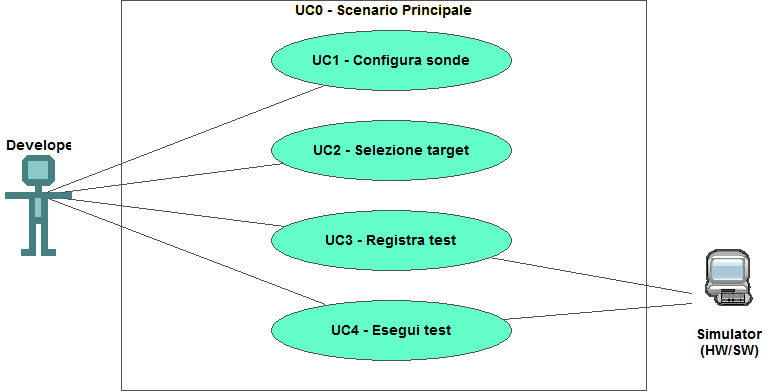
\includegraphics[width=0.9\columnwidth]{usecase/scenario-principale} 
    \caption{Use Case - UC0: Scenario principale}
\end{figure}

\begin{usecase}{0}{Scenario principale}
\usecaseactors{Sviluppatore applicativi}
\usecasepre{Lo sviluppatore è entrato nel plug-in di simulazione all'interno dell'IDE}
\usecasedesc{La finestra di simulazione mette a disposizione i comandi per configurare, registrare o eseguire un test}
\usecasepost{Il sistema è pronto per permettere una nuova interazione}
\label{uc:scenario-principale}
\end{usecase}

\section{Tracciamento dei requisiti}

Da un'attenta analisi dei requisiti e degli use case effettuata sul progetto è stata stilata la tabella che traccia i requisiti in rapporto agli use case.\\
Sono stati individuati diversi tipi di requisiti e si è quindi fatto utilizzo di un codice identificativo per distinguerli.\\
Il codice dei requisiti è così strutturato R(F/Q/V)(N/D/O) dove:
\begin{enumerate}
	\item[R =] requisito
    \item[F =] funzionale
    \item[Q =] qualitativo
    \item[V =] di vincolo
    \item[N =] obbligatorio (necessario)
    \item[D =] desiderabile
    \item[Z =] opzionale
\end{enumerate}
Nelle tabelle \ref{tab:requisiti-funzionali}, \ref{tab:requisiti-qualitativi} e \ref{tab:requisiti-vincolo} sono riassunti i requisiti e il loro tracciamento con gli use case delineati in fase di analisi.

\newpage

\begin{table}%
\caption{Tabella del tracciamento dei requisti funzionali}
\label{tab:requisiti-funzionali}
\begin{tabularx}{\textwidth}{lXl}
\hline\hline
\textbf{Requisito} & \textbf{Descrizione} & \textbf{Use Case}\\
\hline
RFN-1     & L'interfaccia permette di configurare il tipo di sonde del test & UC1 \\
\hline
\end{tabularx}
\end{table}%

\begin{table}%
\caption{Tabella del tracciamento dei requisiti qualitativi}
\label{tab:requisiti-qualitativi}
\begin{tabularx}{\textwidth}{lXl}
\hline\hline
\textbf{Requisito} & \textbf{Descrizione} & \textbf{Use Case}\\
\hline
RQD-1    & Le prestazioni del simulatore hardware deve garantire la giusta esecuzione dei test e non la generazione di falsi negativi & - \\
\hline
\end{tabularx}
\end{table}%

\begin{table}%
\caption{Tabella del tracciamento dei requisiti di vincolo}
\label{tab:requisiti-vincolo}
\begin{tabularx}{\textwidth}{lXl}
\hline\hline
\textbf{Requisito} & \textbf{Descrizione} & \textbf{Use Case}\\
\hline
RVO-1    & La libreria per l'esecuzione dei test automatici deve essere riutilizzabile & - \\
\hline
\end{tabularx}
\end{table}%


\section{Adattamento degli operatori preesistenti}
Durante l'analisi dei requisiti relativa alla nuova funzionalità, sono sorti dei problemi relativi all'adattabilità degli operatori preesistenti con la nuova funzionalità creata. Tali problemi di adattabilità si possono riassumere in micro-aree:

\begin{itemize}
	\item{adattabilità della rappresentazione degli eventi tramite l'ouput dell'operatore \textbf{Bumblebee} definito come \textbf{BumblebeeOuput}, che va a definire la trasformazione degli eventi "grezzi" in eventi arracchiti da informazioni necessarie per il loro processamento;}
	\item{adattabilità dell'\textbf{operatore di windowing} che ora non devo solo trattare aggreazione di eventi ricevuti dallo stesso tipo di risorsa, ma deve gestire l'aggregazione e/o l'allineamento anche di risorse di tipo differente per permettere all'operatore di \textit{Anomaly Detector} di eseguire un controllo a livello di insieme relativo a risorse differenti;}
	\item{adattabilità dell'operatore \textbf{Anomaly Detector} per permettere ad esso di gestire e di controllare gruppi di eventi derivanti da risorse non più eguali fra di loro. Quindi di gestire il controllo relativo alla presenza di una anomalia relativa ad un gruppo di risorse. Inoltre, tale operatore, deve adattarsi anche alla presenze di due nuovi \textit{detector} di anomalie, quali \textbf{Unsupervised} e \textbf{Rule based}.}
\end{itemize}
	
Nello specifico si va ad analizzare le modifiche adottate riguardo le tre micro-aree descritte precedentemente.

\subsection{BumblebeeOutput}\label{sec:bbout}
Per permettere la rappresentazione di gruppi di risorse differenti, viene cambiata la struttura dell'output dell'operatore \textbf{Bumblebee}, rappresententato inizialmente in un formato \gls{json} così rappresentato:

\begin{minted}{js}
{
  "id": // id dell'evento, generato o trasformato dall'evento originale, in formato String,
  "pipeID": // id della pipeline, in formato String,
  "pipeVersion": //versione della pipeline, in formato String,
  "adapterID": //id dell'adattatore, in formato String,
  "tid": //id del cliente, in formato String,
  "assetID": //id della risorsa, in formato String,
  "ts": //timestamp dell'evento, in formato String,
  "asset": //informazioni relative alla risorsa dopo che è stata arricchita, in formato AssetInfo
  "data": //payload dei dati dell'evento trasformati in formato JSON,
  "ctxData": //dati relativi al contesto, come per esempio il tempo metereologico, in formato JSON,
  "meta": //metadati arricchiti dall'operatore di anomaly detection, in formato Option[EventMeta],
  "type": //tipo di BumblebeeOutput", in formato Option[String],
  "srcID": //id della fonte dell'evento in formato String
}
\end{minted}

Dopo l'opportuna modifica, la struttura rappresentate il \textbf{BumblebeeOutput} è così formata:

\begin{minted}{js}
{
  "id": // id dell'evento, generato o trasformato dall'evento originale, in formato String,
  "pipeID": // id della pipeline, in formato String,
  "pipeVersion": //versione della pipeline, in formato String,
  "adapterID": //id dell'adattatore, in formato String,
  "tid": //id del cliente, in formato String,
  "object": {
	  "id": //id dell'oggetto, in formato String,
	  "type": //tipo dell'oggetto rapresentanto (asset,category,group), in formato String
  }
  "ts": //timestamp dell'evento, in formato String,
  "asset": //informazioni relative alla risorsa dopo che è stata arricchita, in formato AssetInfo
  "data": //payload dei dati dell'evento trasformati in formato JSON,
  "ctxData": //dati relativi al contesto, come per esempio il tempo metereologico, in formato JSON,
  "meta": //metadati arricchiti dall'operatore di anomaly detection, in formato Option[EventMeta],
  "type": //tipo di BumblebeeOutput", in formato Option[String],
  "srcID": //id della fonte dell'evento in formato String
}
\end{minted}
dove la rappresentazione è slegata da un \textit{asset} (risorsa) specifico. Per cui l'output sarà adattato ad un \textit{oggetto} generale, rappresentato da un proprio \textbf{id} e da un suo \textbf{tipo}.
Tale struttura finale garantisce una corretto processamento del dato nel caso in cui si tratti di una risorsa singola oppure di un raggruppamento di quest'ultime.
\subsection{Operatore di windowing}
L'\textbf{operatore di windowing} serve per rappresentare un determinato evento in una data finestra temporale. Inizialmente, tale operatore, trattava l'aggregazione solo di una determinata \textit{risorsa} su se stessa, cioè \textit{sommando} o \textit{mediando} un determinato valore. Ora in tale operatore non solo permane il comportamento appena descritto, ma è presente anche la funzionalità che si occupa di allineare e/o aggregare fra di loro \textit{risorse} di tipo differente, per permettere un processamento dei dati a livello collettivo. Per definire il comportamento dell'operatore di windowing, è necessaria un apposita \textbf{configurazione} che sarà iniettata durante il processamento attivo dei dati, per permetterne la modifica del comportamento senza dover riavviare l'intero applicativo e creare uno stallo in esso.\\
Il flusso attuale dell'operatore prevede questi step:

\begin{enumerate}
	\item{arrivo dell'\textit{evento} di tipo \textit{BumblebeeOutput};}
	\item{controllo relativo a se la configurazione è settata, nel caso si saltano tutti i passaggi successivi;}
	\item{le varie risorse vengono aggregate su se stesse;}
	\item{nel caso serva un'aggregazione a gruppi, è presente una mappa fra l'\textit{id del gruppo} (fornito dalla configurazione o creato da essa) e l'\textit{aggregatore delle risorse}, questo per permettere di avere un'aggregazione suddivisa in gruppi e di non andare ad intaccare aggregatori che possono trattare logicamente le stesse risorse, ma in gruppi differenti;}
	\item{viene aggiornata la mappa descritta nel punto precedente con l'aggiunta dell'aggregatore basandoci sull'\textit{id del gruppo}. Nel caso l'id del gruppo non sia presente, viene creata una nuova \textit{entry} all'interno della mappa e salvato l'opportuno aggregatore;}
	\item{quando scade il \textit{timer} della window, verrà processata l'aggregazione secondo le indicazioni date dalla configurazione, producendo l'ouput descritto nella sezione \S\textbf{OutputWindow}}.
\end{enumerate}

\myParagraph{OutputWindow}
L'ouput dell'operatore, dapprima rappresentava solo una \textbf{risorsa singola}, ora invece tratterà un \textit{gruppo}, il quale è identificato da un \textbf{id}, da un \textbf{\gls{timestamp}} e da un \textbf{array} di \textit{risorse} di tipo \textit{BumblebeeOutput}.\\
L'OutputWindow può rappresentare logicamente tre tipi logici di dato:
\begin{itemize}
	\item{\textbf{elemento singolo:} dove l'\textit{array} degli eventi è formato \textit{1} elemento, l'\textit{id del gruppo} equivale all'id della risorsa dell'unico evento all'interno dell'array e il \textit{\gls{timestamp}} equivale al \gls{timestamp} dell'unico evento all'interno dell'\textit{array};}
	\item{\textbf{singolo elemento aggregato:} dove l'\textit{array} degli eventi è formato da \textit{1} elemento, l'\textit{id del gruppo} equivale all'id definto dalla configurazione e il \textit{\gls{timestamp}} equivale a quello definito durante l'aggregazione effettiva;}
	\item{\textbf{allineamento:} dove l'\textit{array} degli eventi è formato da \textit{N} elementi, l'\textit{id del gruppo} equivale all'id definto dalla configurazione e il \textit{\gls{timestamp}} equivale a quello definito durante l'aggregazione effettiva;}
\end{itemize}



\subsection{Anomaly Detector}
L'operatore \textbf{Anomaly Detector} è colui che si occupa di sollevare segnalazioni nel caso sia presente un'anomalia riguardo l'evento entrante (di tipo \textbf{OutputWindow}). Dapprima il l'Anomaly Detector lavorava solo su un tipo di evento legato ad una \textit{risorsa} singola, mappando l'\textit{id del detector} ad un'altra mappa dove la chiave è rappresentata dall'\textit{id della risorsa} e il valore è rappresentato dal vero e proprio \textit{detector}. Ora invece la struttura è basata sull'\textit{id del gruppo}, per cui è stata creata un'ulteriore mappa fra \textit{id del gruppo} e \textit{id del detector}, inoltre la chiave della mappa interna non è più rappresentata da un'id della risorsa, ma da un \textit{id dell'oggetto} dopo la modifica di \textbf{BumblebeeOutput} \S\ref{sec:bbout}.\\
I \textit{detector} ora avranno un parametro in più che permette di definire se un determinato detector valuta l'anomalia su un gruppo di risorse o su una risorsa singola.\\
Di seguito la lista dei detector:
\begin{itemize}
	\item{\textbf{Uniseas}: detector che lavora singolarmente su un tipo di risorsa;}
	\item{\textbf{Crosscorel}: detector che lavora singolarmente su un tipo di risorsa e su un evento esterno ad essa (come per esempio il tempo metereologico);}
	\item{\textbf{Siblings}: detector che lavora singolarmente su un tipo risorsa valutando il suo andamento su \textit{N} risorse uguali ad essa. Utilizza un algoritmo di \textit{\gls{Apprendimento automatico}} di tipo \textit{\gls{Apprendimento supervisionato}};}
	\item{\textbf{Unsupervised}: detector che lavora su un gruppo di risorse lavorando con un algoritmo di \textit{\gls{Apprendimento automatico}} di tipo \textit{\gls{Apprendimento non supervisionato}};}
	\item{\textbf{Rule based}: detector che lavora su un gruppo di risorse oppure su una risorsa singola in base alla propria configurazione e valutando l'andamento della/e risorsa/e tramite una regola definita dall'utente.}
\end{itemize}

La modifica apportata al codice sostanzialmente tratta il controllo da effettuare (in base alla \textit{configurazione} del detector) per definire su quale dato processare l'anomalia, nel caso avvenga. Infatti nel caso di un gruppo verrà creato un evento rappresentante tale gruppo su cui sollevare l'anomalia, invece nel caso di una risorsa singola l'anomalia verrà sollevata sull'evento relativa ad essa. 
